\section{Isotropic\_Sqw: A general $S(q,\omega)$ coherent and incoherent scatterer}
\label{s:isotropic-sqw}
\index{Samples!Coherent and incoherent isotropic scatterer}
\index{Coherent and incoherent isotropic scatterer}
\index{Inelastic scattering}

\component{Isotropic\_Sqw}{V. Hugouvieux, E. Farhi}{Sqw$\_{coh}$, $\sigma_{coh}$, Sqw$\_{inc}$, $\sigma_{inc}, V_\rho, \sigma_{abs}, T$}{$q_{min}, q_{max}, \omega_{min}, \omega_{max}, d\phi$, order}{not fully validated}

\begin{figure}
  \begin{center}
    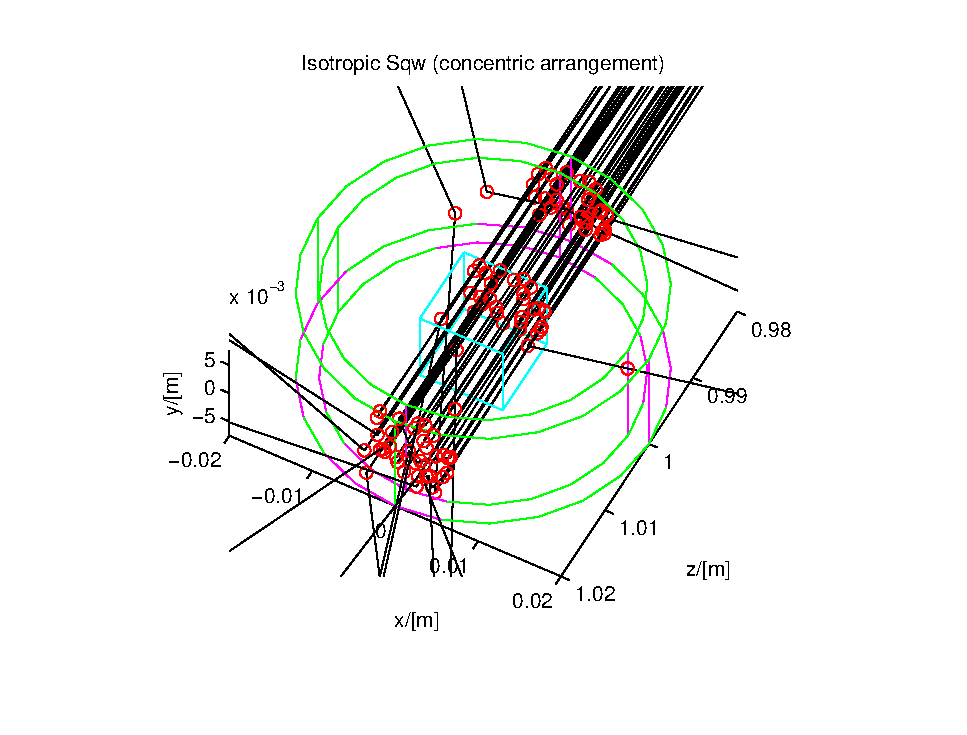
\includegraphics[width=0.9\textwidth]{figures/sqw.eps}
  \end{center}
\caption{An $l-^4$He sample in a cryostat, simulated with the Isotropic\_Sqw component in concentric geometry.}
\label{f:isotropic-sqw}
\end{figure}

The component assumes that the sample has the structure of an isotropic material. This stands for liquids, glasses (amorphous systems), polymers, gaz, and may be extended to powders.

\subsection{Neutron interaction with matter}

When a neutron enters a material, according to usual models and letting the absorption aside to begin with, it 'sees' atoms as disks with a surface equal to the total scattering cross section of material $\sigma$. Each coherent and incoherent process is associated with a given probability to hit these cross-sections, according to $\sigma_{coh}$ or $\sigma_{inc}$. We may choose randomly a scattering position along the path, using e.g. an expeonential decay probability. If the scattering condition is not satisfied, the neutron is transmitted, and leaves the sample. In any case, the absorption lowers the intensity according to an $e^{-\rho \sigma_{abs}d}$ absorption law along the propagation path $d$. In this process, the neutron is considered to be a particule.

Once the neutron 'knows' that something (terrible) is going to occur, it looks for a possible excitation to interact with. Then we turn to the wave description of the neutron, which interacts with the whole volume. The distribution of excitations, from which derives their relative intensity in the scattered beam, is simply the dynamic structre factor - or scattering law - $S(q,\omega)$. According to the definition of the density of states, we may use $g(\omega)$ as the probability law to scatter at a given energy transfer.

The neutron leaves the scattering point when a suitable $(q, \omega)$ choice has been found to satisfy the conservation laws. The process is iterated until the neutron leaves the volume of the material, eventually producing multiple scattering contributions.

\subsection{Theoretical side}

Following Squires (\cite{squires}, p63), the neutron differential scattering cross section for both coherent and incoherent processes is
\begin{equation}
\frac{d^2\sigma}{d\Omega dE_f} = \frac{\sigma}{4\pi}\frac{k_f}{k_i} N S(q, \omega)
\end{equation}
with usual notations: $N=\rho V$ is the number of atoms in the scattering volume $V$ with density $\rho$, $E_f, E_i, k_f, k_i$ are the energy and wavevectors of final and initial states respectively, and $\sigma$ is the total scattering cross-section. The unit of the dynamical structure factor $S(q,\omega)$ is an inverse energy.

Some easely measureable quantities in a liquid are the \emph{static pair correlation function} $g(r)$ and the \emph{structure factor} $S(q)$, defined as:
\begin{eqnarray}
\rho g(\vec{r}) &=& \frac{1}{N} \sum_{i=1}^N \sum_{j \neq i} \langle \delta(\vec{r}+\vec{r}_i-\vec{r}_j) \rangle \\
S(\vec{q}) &=&\int S(\vec q,\omega) d\omega \\
           &=&1 + \rho \int_V [g(\vec{r})-1] e^{i\vec{q}.\vec{r}} d\vec{r} \\
           &=&1 + \rho \int_{0}^{\infty} [g(r)-1] \frac{\sin(qr)}{qr} 4 \pi r^2 dr {\rm\ in\ isotropic\ materials.}
\end{eqnarray}
Both $g(r)$ and $S(q)$ converge to unity for large $r$ and $q$ values respectively, and they are representative of the atoms spatial distribution. Moreover in a liquid $\lim_{q \rightarrow 0} S(q) = \rho k_B T \chi_T$ where $\chi_T=\frac{\partial \rho}{\partial P}_{V,T}$ is the compressibility \cite{Egelstaff67}. These quantities are obtained experimentaly from diffractometers.

On the other hand, we may measure, usually with time-of-flight instruments, the \emph{density of states} $g(\omega)$  which is the fraction of modes whose energy lie between $\omega$ and $\omega+d\omega$ \cite{lovesey84}
\begin{equation}
g(\omega) = \frac{\int S(q,\omega) dq}{\iint S(q,w) dq, d\omega} .
\end{equation}
This function is normalized to unity, $\int g(\omega) d\omega = 1$ and is a probability distribution of mode energies in the material.

The main idea to implement the scattering from $S(q, \omega)$ is to basically make two consecutive Monte Carlo choices, applying the well known \emph{joint probability} theorem:
\begin{equation}
\label{eq:jointproba}
P(q \cap \omega) = P(\omega).P(q \mid \omega) .
\end{equation}

Thus we define $P(\omega)$ as the cumulated distribution of the density of states $g(\omega)$.  $P(\omega)$ is the probability for an excitation to have an energy lower than $\omega$.

Similarly, we define the conditional probability $P(q \mid \omega)$ to be, for each energy lying between $\omega$ and $\omega+d\omega$, the cumulated distribution of
\begin{equation}
\hat g(q\mid\omega) = \frac{S(q, \omega)}{\int S(q,\omega) dq} .
\end{equation}
This latter is the density of wavevector transfers for a selected energy transfer, and
$P(q \mid \omega)$ is the probability for an excitation to have a wavevector lower than $q$, for a given energy transfer $\omega$.

\begin{figure}
  \begin{center}
    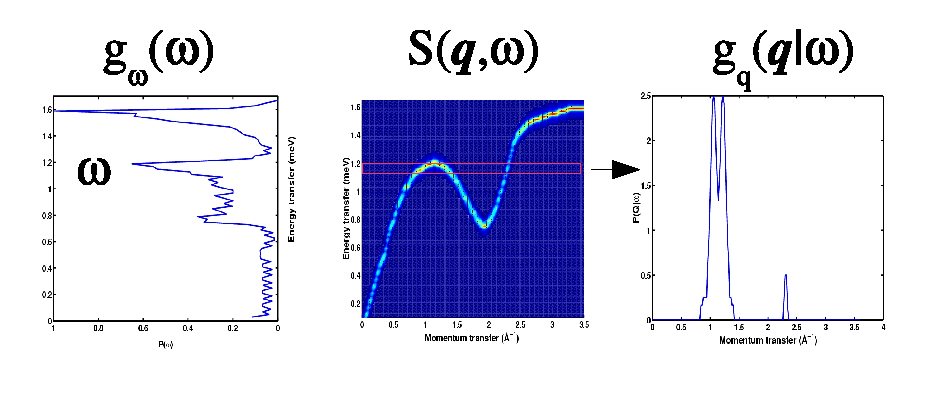
\includegraphics[width=0.9\textwidth]{figures/Sqw_sampling.eps}
  \end{center}
\caption{The probability functions extracted from $S(q,\omega)$. The energy transfer is first selected from the density of states, then the wavevector is obtained from $\hat g$.}
\label{f:isotropic-sqw}
\end{figure}


\subsection{The implementation}

\subsubsection{Choosing the interaction type}

The method used is similar to the one adopted in the \verb+Single_crystal+ component (section \ref{s:Single_crystal}).

We first compute the absorption and total cross-section
\begin{eqnarray}
\sigma_{abs} &=& \sigma_{abs}^{{\rm 2200~m/s}}\frac{2200 m/s}{v} \\
\sigma_{tot} &=& \sigma_{abs} + \sigma_{coh} + \sigma_{inc}
\end{eqnarray}
as well as the neutron trajectory intersection with the geometry. This provides the total path length in the sample $d_{out}$ to the exit.
Defining the linear attenuation $\mu = \rho\sigma_{tot}$, the probability that the neutron scatters (or be absorbed) along path $d_{out}$ is $e^{-\mu d_{out}}$. If this condition is not satisfied, the neutron leaves the sample unchanged.
In the other case, we adjust the neutron weight by a factor $\frac{\sigma_{coh} + \sigma_{inc}}{\sigma_{tot}}$ to account for the portion of absorbed neutrons along the path.
Additionally, we choose randomly the type of interaction with fractions $\sigma_{coh}$ and $\sigma_{inc}$.

\subsubsection{Choosing the interaction position}

If the straight path to the sample volume exit is $d_{out}$, the probability that the neutron scatters before exiting the sample at a distance $d_{scatt}$ is:
\begin{equation}
P(d_{scatt} < d_{out}) = \int_0^{d_{out}} \mu e^{-\mu x}dx = 1 - e^{-\mu d_{out}}. \\
\end{equation}
Form that law, we may compute the cumulated distribution, which gives the probability for scattering to occur at a distance lower than $d_{scatt}$, knowing that the neutron interacts before $d_{out}$. This law may be analytically inverted so that the path length $d_{scatt}$ may be obtained directly from a uniform distribution random number $\xi$
\begin{equation}
d_{scatt} = -\frac{1}{\mu} \ln(1 - \xi[1 -e^{-\mu d_{out}}]).
\end{equation}

\subsubsection{Choosing the $q$ and $\omega$ transfer}

If no $S(q, \omega)$ data is available and the scattering process has been chosen as incoherent, we set $\omega=0$ and select randomly an outgoing wave vector $\boldsymbol{k}_f$.

In case the $S(q, \omega)$ data is available for the scattering process (coherent or incoherent), a random choice is made to select the energy transfert using $P(\omega)$ with the $g(\omega)$ probability distribution.
Similarly, we use $P(q \mid \omega)$ to select a wavevector transfer.

Chosing a $(q, \omega)$ set and applying Eq. (\ref{eq:jointproba}), we have obtained a probabilistic nomalized evaluation of the dynamical structure factor, which we multiply by the norm $|S| = \iint S(q,\omega) dq d\omega$ to obtain $S(q, \omega)$:
\begin{equation}
S(q, \omega) = |S|. P(\omega).P(q \mid \omega) .
\end{equation}

Then a selection between energy gain and loss is done with the detailed balance ratio $e^{-\hbar \omega / k_B T}$.

\subsubsection{Choosing the scattered wave vector}

The next step is to check that conservation laws (\ref{eq:q-transfert}) and (\ref{eq:w-transfert}) can be satisfied. These conditions are closely related to the method for selecting the outgoing wave vector direction.

When the final wave vector has to be computed, the quantities $\vec{k}_i$, $\hbar \omega$ and $q = |\vec{q}|$ are known.
From the energy conservation law Eq. (\ref{eq:w-transfert}), we select ramdomly one of the two roots, $k_f^+$ and $k_f^-$.
The scattered wave vector is noted : $\vec{k}_f = k_f \vec{\hat k}_s$ where $\vec{\hat k}_s$ is a unit vector.\\
Since we only know the norm of the scattering vector $\vec{q}$, the momentum conservation law Eq. (\ref{eq:q-transfert}) may be expressed as
\begin{align}
q^2 = |\vec{k}_i -\vec{k}_f|^2 = |k_i^2 + k_f^2 - 2 k_f \vec{k}_i \cdot \vec{\hat k}_s
\end{align}
where $\vec{k}_i \cdot \vec{\hat k}_s$ stands for the dot product of the vectors.\\
Now, we should solve :
\begin{align}
\vec{k}_i \cdot \vec{\hat k}_s &= \frac{1}{2k_f} (k_i^2 + k_f^2 - q^2) = C \\
|\vec{\hat k}_s| &= 1
\end{align}
where $C$ is a constant.
$\vec{\hat k}_s$ can be decomposed as : $\vec{\hat k}_s = B \vec{k}_i + \vec{u}_0$ where $B$ is a constant and $\vec{u}_0$ is a vector of $Vect(\vec{k}_i)^{\bot}$ (that is the orthogonal of the space generated by $\vec{k}_i$), which is a plane $P$.
Since we have : $\vec{k}_i \cdot \vec{\hat k}_s = C$, we may write : $B = \frac{C}{k_i^2}$.
\begin{figure}[!h]
\begin{center}
\includegraphics*[height=6cm]{figures/calckf_2.eps}
\caption{How to compute the outgoing wavevector direction $\vec{\hat k}_s$}
\label{fig:ann_kf}
\end{center}
\end{figure}
The vectors $\vec{u}_0$ such that $|\vec{\hat k}_s| = 1$ define a circle of radius $R$ : $|\vec{u}_0|~=~R$.
Since $\vec{u}_0$ and $B \vec{k}_i$ are orthogonal, we find :
\begin{align}
\frac{C^2}{k_i^2} + R^2 = |\vec{\hat k}_s|^2 = 1
\end{align}
from which we deduce the radius of the circle :
\begin{align}
R = \sqrt{1 - \frac{C^2}{k_i^2}}.
\end{align}
Let us now define an orthonormal basis ($\vec{u}_1,\vec{u}_2$) of the plane containing $\vec{u}_0$.
$\vec{u}_0$ can be decomposed as : $\vec{u}_0~=~R(\cos \theta \vec{u}_1 + \sin \theta \vec{u}_2)$, where $\theta$ can be randomly drawn for a uniform distribution.
Finally, we obtain :
\begin{align}
\vec{\hat k}_s = \frac{C^2}{k_i^2} \vec{k}_i + R (\cos \theta \vec{u}_1 + \sin \theta \vec{u}_2)
\end{align}

\subsubsection{Important remarks}

Since the choice of the interaction type, we know that the neutron \emph{must} scatter, with an appropriate $\vec k_f$ outgoing wave vector. If any of the choices in the method fails:
\begin{enumerate}
\item the roots $k_f^+$ and $k_f^-$ are imaginary, which means that conservation laws can not be satisfied and for instance the selected energy transfert is higher than the incoming neutron energy
\item the radius of the target circle $R$ is imaginary
\end{enumerate}
then a new $(q, \omega)$ set is drawn, and the process is iterated until sucess or - at last - removal of the neutron event. This latter absorption is then reported at the end of the simulation, as it never occurs in reality (neutrons that scatter do find a suitable $(q, \omega)$ set).\index{Removed neutron events}

A way to avoid this is to focus the $q,\omega$ range from the $S(q, \omega)$ data file to the actual beam characteristics. This is done by setting the component parameter $wmax$ to the maximum energy of the incoming beam.

Selecting the whole $q$ and $\omega$ range, to the one being able to scatter the incoming beam, when using the component does improve significantly the speed of the computation. Additionally, if you restrict the scattering the first order only (parameter order=1), then you may specify the angular vertical extension $d\phi$ of the scattering area to gain optimized focusing. This option does not apply when handling multiple scattering (which emits in $4\pi$ many times before exiting the sample).

